%%=============================================================================
%% H3 - Ontwerpprincipes van ZFS
%%=============================================================================

\chapter{Ontwerpprincipes \& architectuur van ZFS}
\label{ch:h3}

In dit hoofdstuk worden enkele principes besproken waarop de ontwikkelaars zich hebben gebaseerd bij het ontwerp en de onwtikkeling van ZFS. Tevens wordt de architectuur van ZFS reeds globaal beschreven, om zo de ontwerpbeslissingen van de ontwikkelaars wat meer toe te lichten.

\section{Ontwerpprincipes}

De principes die aan de basis van ZFS liggen vloeiden meestal voort uit de problemen die de ontwikkelaars zelf ervaarden bij het gebruik van andere bestandssystemen.

\subsection{Eenvoud van beheer \& Storage Pools}

Volgens \textcite{ZFSBonwick} kan en moet het aanmaken en beheren van bestandssystemen een stuk makkelijker gemaakt worden. Hierbij speelt automatisatie van verschillende taken een belangrijke rol. Het doel van de gebruiker, nl. \textit{"Het aanmaken van een bestandssysteem"} zou moeten worden vooropgesteld; tevens moet dit proces zo snel een eenvoudig mogelijk verlopen. Ook moet het mogelijk zijn om beheerderstaken (zoals bestandssystemen aanmaken en verwijderen) uit te voeren zonder de werking van het gehele systeem te ondermijnen \autocite{ZFSBonwick}. 

Een niet onbelangrijke feature hierbij zijn storage pools. Storage pools hebben als doel om opslagruimte zoveel mogelijk los te koppelen van de fysieke schijven: alle schijven bevinden zich in een pool van disks. Uit deze pool kunnen bestandssystemen worden aangemaakt, zonder rekening te moeten houden met de limitaties van bv. partities. Tevens kunnen bestandssystemen op een flexibele manier gebruik maken van deze pooled storage door automatisch in te krimpen en uit te breiden wanneer nodig \autocite{ZFSBonwick}. 

\begin{figure}
        \centering
        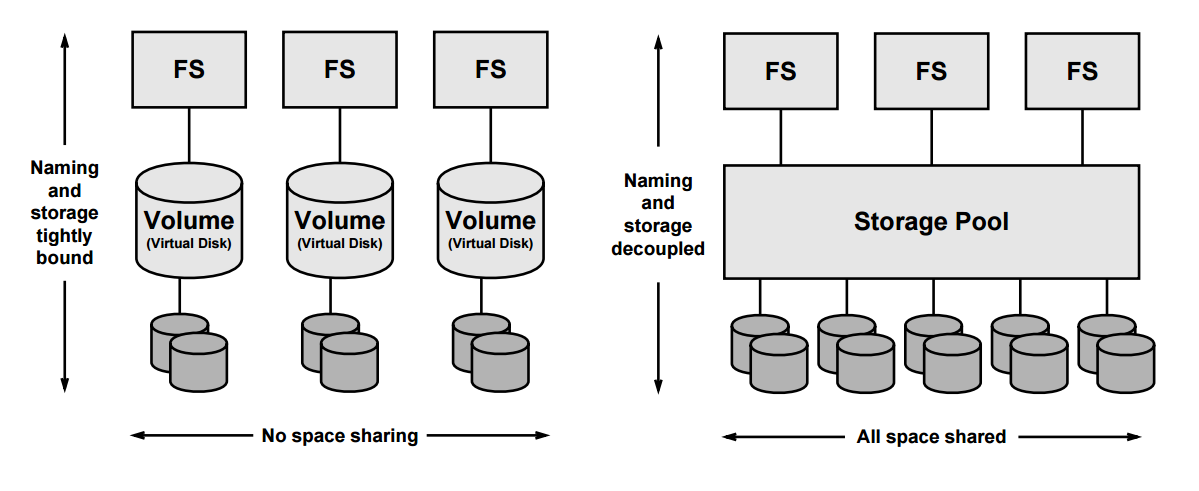
\includegraphics[width=0.8\textwidth]{h3-pools-vs-vols}
        \caption{Illustratie van ZFS pooled storage (rechts) t.o.v.volume-based storage (links) \autocite{ZFSBonwick}}
        \label{fig:bonwick_pools_illustratie}
\end{figure}

\subsection{Consistentie \& Integriteit}

Eén van de taken van een bestandssysteem is om ervoor te zorgen dat het in een consistente toestand blijft, i.e. het moet mogelijk zijn om van inconsistente toestanden te herstellen d.m.v. bijvoorbeeld een journal of door een filesystem check te draaien \autocite{OSThreePiecesRemzi2015}. Een nadeel aan deze technieken volgens \textcite{ZFSBonwick} is dat deze niet makkelijk zijn om te implementeren, omdat bijvoorbeeld in het geval van journaling filesystems een roll back of roll forward moet worden uitgevoerd. Hierbij moet ook nog de volgorde van de bewerkingen in acht worden genomen \autocite{OSThreePiecesRemzi2015}. 

De oplossing volgens \textcite{ZFSBonwick} is om het bestandssysteem te allen tijde consistent te houden; er mag m.a.w. geen enkel moment zijn waarop het file system in een inconsistente toestand terecht komen. Dit wordt verwezenlijkt door de Copy-On-Write eigenschappen ZFS, waardoor bewerkingen atomair gebeuren \autocite{ZFSBonwick}.


